
\section{Multilayer Network}

In this section we will dive into all the unexplored paths, starting from falkenberg work. In particular we will do the same polarization analysis on a topic level, instead of computing it at a full network level, we created  a retweet network for each topic, so we can see which are the topics that are driving the polarization of cop. Furthermore we also want to explore how the polarization of topics evolved during the time.

Thanks to the previous section now we are familiar with the concept of topic modeling and how the main models perform, now the goal is to create a multilayer network where each layer is represented by a topic. 

In order to to so we developed a python library  that can be used as a toolbox starting from the tweets fresh out from the official API of Twitter. The design is modular and can achieve different goals.
In fact even if we are interested only in the retweet network of the users (nodes are users, ties are retweets), this framework can be used to: 

\begin{itemize}
    \item Labeling tweets according to their topic
    \item Create a temporal text network 
    \item Create the retweet network (normal and multilayer version)
    \item Create the reply network
    \item Create the quote network

\end{itemize}

The steps are independent, so, for example, you can also create the network without the need to run the topic modeling part.

\paragraph{Steps}
Even though you can skip some steps and start with your own data, the natural and minimal pipeline follow these steps:


\begin{enumerate}
    \item from json to a tabular format 
    \item label each tweet with a topic
    \item create multilayer retweet network  
    
\end{enumerate} 


\subsection{Process input}

The first step consists of the transformation of the json objects into tabular data to optimize the space and handle the data in an easier way with pandas. In this process all the tweets with attachments and not in English are discarded, then the tweets are divided into multiple dataframes, one for original tweets, i.e. the ones that are actively written by the author, and one for retweets.

At the end of this stage, a csv and pkl file are saved in case somebody needs the tweets in tabular data. Also for caching porpuses, in fact in you rerun the script and these file exists they will be loaded.

\subsection{Topic modeling}

As we extensively discussed in chapter \ref{Ch:related} in this segment of the pipeline, the tweets can be labeled using Bertopic, with the possibility to choose the embedder, the one used in this research is \textit{all-MiniLM-L6-v2} .

This step is the most computationally expensive, for this reason, to avoid redundancy, the topic modeling has been run only to original tweets. 

After this step, all the original tweets are labeled with a topic, and then the label has been propagated to all the retweets so that the entire dataset is now labeled with a topic.

At this point it is possible to use the OpenAI API to give a meaningful label to the topics, before this it was just the most relatively frequent words of the topic. Using the langchain library it is possible to structure a prompt to be used. this is the one I used: 
\\

\textit{    I want you to act as a tweet labeler, you are given representative words
from a topic and three representative tweets, give more attention to the words, all the tweets are related to climate change, and COP, no need to mention it, detect subtopics.
start with "label:" and avoid hashtags,
which is a good short label for the topic containing the words [{words}], here are 3 tweets to help you:
first = "{tweet1}", second = "{tweet2}", third = "{tweet3}}
\\

Similarly to the previous stage, the labeled dataset is saved in the cache folder both in csv and pkl. The model is saved too

\subsection{Temporal text network}
\textit{should i add this chapter?}

This step creates a temporal text network according to Vega and Magnani \cite{vega_foundations_2018} 

The input of this stage is the dataframe containing all the tweets just created, but due to its modularity, you can use your own.

There are 2 kinds of nodes: users and tweets

there are 3 kinds of edges : 
\begin{itemize}
    \item \textbf{user-tweet}: if the user has tweeted the tweet
    \item  \textbf{tweet-user}: if the tweet mention the user
    \item \textbf{tweet-tweet:} if the tweet retweets the other
\end{itemize}


The method returns also two dictionaries that map tweet nodes to their text and edges to their timestamp, this information is also stored as attributes in the network.
\begin{figure}
    \centering
    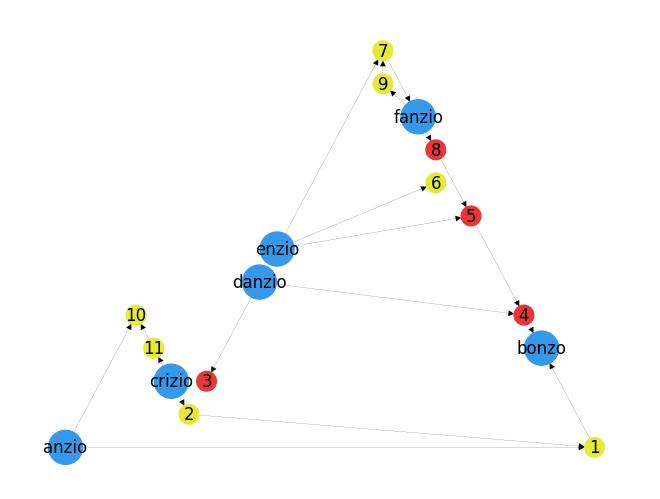
\includegraphics[width=0.75\linewidth]{Chapter4/figures/full_network.png}
    \caption{This is a visualization of a temporal text network, the bigger nodes are the users, the smaller are the tweets, and the color is the topic}
    \label{fig:tt_network}
\end{figure}

The graph is stored in GML format in the network folder

\subsection{Project the network}
The temporal text network contains much information and can be used for many different projects, but sometimes having a simpler data structure is more helpful.

To simplify the analysis we want to have only one set of nodes, the authors, and see how they are related: this process is known as projection. The network is directed and the rules for connecting the users are the following:
\begin{itemize}
    \item if user a is retweeting a tweet of user b : $a \rightarrow  b $
    \item if user c mentions d in a tweet: $ c \rightarrow d $
\end{itemize}


Generally, a tie between two users means that the first did an action towards the second, the action can be a retweet or a mention.

This is achieved using a hybrid approach using both iteration and recursion: first, it iterates over all the users, and for each user iterates on all its tweet then it recursively search for the end of the retweet chain.

All the ties take into account the topic of the tweets, so multiple networks are created at this point, one for each topic, all saved in GML format.


\subsection{Retweet network}
While the projection of the temporal text network creates an interaction network, so including both retweets and mentions, it is also possible to create the pure retweet network. 
The network is directed, the nodes are the users, the tie is the number of retweets. For each topic a network is created.

\subsection{Multilayer network}

The last step is the creation of a multilayer network using the multinet library developed by Uppsala University, at this point all the different networks created in the previous step are merged into a multilayer network

\begin{figure}
    \centering
    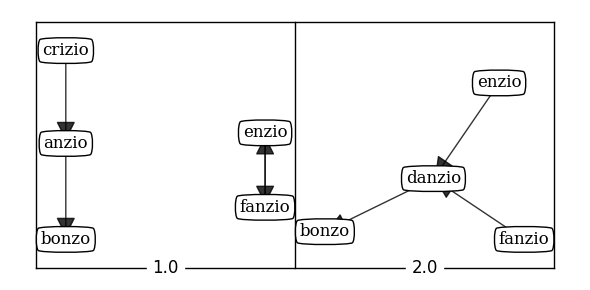
\includegraphics[width=0.75\linewidth]{Chapter4/figures/projected_topics_ml.png}
    \caption{Example of multilayer retweet network \ref{fig:tt_network}}
    \label{fig:multilayer}
\end{figure}



In the process of the creation of the network there are retweeted tweets that do not have the original one, so we discard them.

\section{Polarization}
At this point, for each layer, we can compute for each user a latent ideology score, and then using the hartigan's diptest, we can assign to each topic a polarization value. More the datails on how this is computed is in the related work.
In these process there are some parameters we can adjust, the number of influencer andn (to explain)

Now we have for each user a list of topics he tweeted and the ideology score for each of them.

\section{Logitudinal analysis}
In order to see topic polarization over the time we need to run the topic modeling with all the tweets, but they are too many, so instead of taking the original tweet of cop 21 and cop26, we only take the one with retweets which are around 1/3 of the total but are the one needed to be propagated to the rest of the network

\paragraph{Getting top influencer}
The top n influencers are simply the n influercers with the highest indegree in the retweet network, i.e. the most retweeted ones.


After doing this process for all the cops, the dataframes are merged and saved.

\paragraph{get topics}
At this point we can run the topic modeling on the original tweets and then propagate the results to the retweets 
